\subsection{Standard Signals}
To validate the iPad application, the prototype was tested with standard signals. The voltage applied to each input pin is summarised in Table~\ref{table: standard signals}. The A0 pin on the Arduino, corresponding to glucose, was tested with a random noise signal. The A1 pin, corresponding to lactate, was tested with a square wave. The A7 pin, corresponding to potassium, was tested with a sine wave. 

\begin{table}[h!]
\centering
\begin{tabular}{||c c c||} 
 \hline
 Input Pin & Neurochemical & Signal Description \\ [0.5ex] 
 \hline\hline
 A0 & Glucose & Noise signal with 1V P-P voltage, 0.5V offset \\
 A1 & Lactate & 0.1Hz square wave, 1V P-P voltage, 0.5V offset \\
 A7 & Potassium & 0.1Hz sine wave, 0.5V P-P voltage, 0.5V offset \\
 \hline
\end{tabular}
\caption{Standard signals received by input pins}
\label{table: standard signals}
\end{table}

The signals were chosen to have a low frequency of 0.1Hz since the neurochemical signals present during the occurrence of an SD display changes slowly and over a long time frame. Furthermore, the app only receives data once every second from each input, hence according the the Nyquist rate, frequencies above 0.5Hz will undergo aliasing and will not be reconstructed well.

The standard signals inputted to the analogue Arduino pins were produced by a signal generator. In parallel, these signals also went to a PicoScope input channel, which was then connected to a laptop so that the signals could be recorded on PicoLog with a sampling frequency of 5Hz. The signals displayed on PicoLog could then be compared with the signals received on the iPad app post processing and transmission. Figure~\ref{fig: test1} shows the set up of the experiment.

\begin{figure}[h!]
\centering
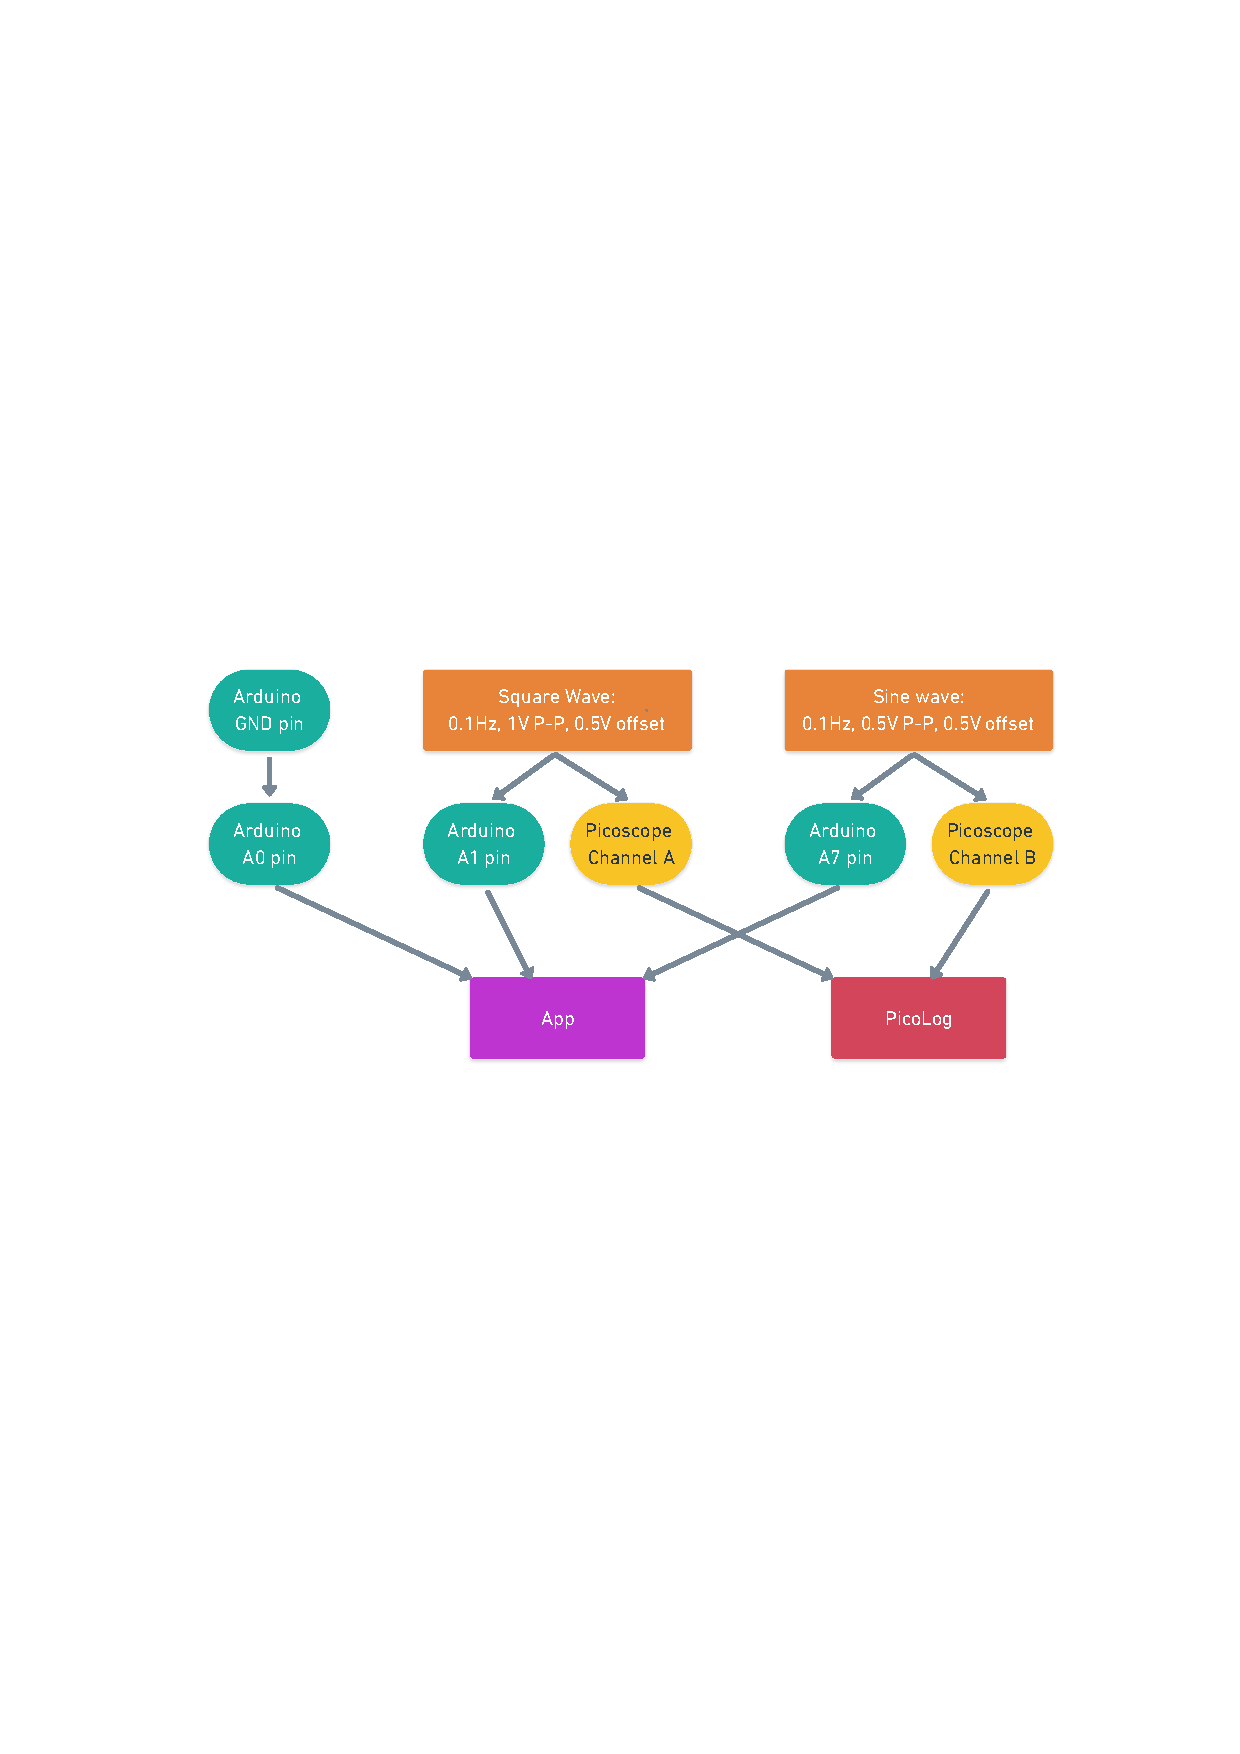
\includegraphics[trim={0cm 0cm 0cm  0cm}, clip, width=.8\textwidth]{./figures/test1.pdf}
\captionsetup{justification=centering}
\caption{Experimental setup for testing standard signals}
\label{fig: test1}
\end{figure}


\subsection{Spreading Depolarisation}
The aim of this test was to see if the characteristics of the SD could be visualised on the app. 18 minutes of potassium, glucose, and lactate patient data sampled at 200Hz, which included the occurrence of an SD, was extracted and downsampled to 50Hz so that the signal was less than 60,000 samples in length in order to be programmed into the Agilent Arbitrary Waveform Generator (AWG). No significant information was lost in the downsampling process as the characteristic components in the signal have frequencies less than 1Hz. The characteristics of the extracted neurochemical signals are shown in Table~\ref{table: patient data}. 


\begin{table}[h!]
\centering
\begin{tabular}{||c c c c c||} 
 \hline
 Neurochemical & P-P Voltage & SD range & Amplification & Processing\\ [0.5ex] 
 \hline\hline
 Glucose & -4.29V -- 6.8V & 0.35V -- 0.7V & No & Yes \\
 Lactate & 0V -- 1.903V & 0V -- 1.903V & No & No \\
 Potassium & 21.59mV -- 79.59mV & 0mV - 20mV & x100 & Yes \\
 \hline
\end{tabular}
\caption{Characteristics of patient data during SD and if processing and amplification were required}
\label{table: patient data}
\end{table}

Since potassium has a low voltage range during an SD and the Arduino is limited to 4.88mV resolution, the signal was multiplied by a 100 for testing purposes so that the Arduino could detect the signal with higher precision. The app accounted for this amplification by dividing the received signal by 100. Potassium and glucose were then processed so that the signals were capped between 0V and 5V, which is the range the Arduino can detect. The signals were then programmed into the AWG. 

Each neurochemical signal was tested one at a time since the AWG is limited to outputting one signal and only one AWG was available to use. The output pin of the AWG was connected to the Arduino input channel on the breadboard depending on which signal was being tested. The other two input channels were connected to ground. Each signal was recorded on the app and then compared to the original patient data.

\begin{table}[h!]
\centering
\begin{tabular}{||c c c||} 
 \hline
 Neurochemical & Concentration (mM) & Voltage (mV) \\ [0.5ex]
 \hline\hline
 Glucose & 0 & 61.5 \\
  & 1 & 137.8 \\
  & 2 & 239.5 \\
 Lactate & 0 & 169.3 \\
  & 0.5 & 622.7 \\
  & 1 & 721.6 \\
 Potassium & 2.7 & -20.2631 \\
  & 6.35 & -0.8875 \\
  & 10 & 9.9214 \\
 \hline
\end{tabular}
\caption{Calibration values obtained from patient data}
\label{table: test2 calibration}
\end{table}

Since real patient data was used for testing, the segmented control switch feature on the app that allows to view the plots as concentration against time could be tested. From the patient data, the nearest calibration occurrence was identified and the calibration values were calculated. The calibration values used in the experiment are shown in Table~\ref{table: test2 calibration} and were inserted in the text fields on the app during testing.

